%%%%%%%%%%%%%%%%%%%%%%%%%%%%%%%%%%%%%%%%%
% ARTIGO PARA A DISCIPLINA DE VISUALIZAÇÃO DE DADOS
%
% Template adaptado por @Gustavo Oliveira.
% Compilação: pdflatex main; bibtex main; pdflatex main; pdflatex main
%%%%%%%%%%%%%%%%%%%%%%%%%%%%%%%%%%%%%%%%%


%% CONFIGURAÇÃO
\documentclass[10pt, a4paper, twocolumn]{article}
%%%%%%%%%%%%%%%%%%%%%%%%%%%%%%%%%%%%%%%%%
% ARQUIVO DE CONFIGURAÇÃO PARA O TEMPLATE DE ARTIGOS DO 
% 'CADERNOS DE VISUALIZAÇÃO DE DADOS'
% http://cdia.ci.ufpb.br
%
% Adaptado por @Gustavo Oliveira.
%
% 
% This file originates from:
% http://www.LaTeXTemplates.com
%
% Authors:
% Frits Wenneker
% Vel (vel@LaTeXTemplates.com)
%
% License:
% CC BY-NC-SA 3.0 (http://creativecommons.org/licenses/by-nc-sa/3.0/)
%
%%%%%%%%%%%%%%%%%%%%%%%%%%%%%%%%%%%%%%%%%

%----------------------------------------------------------------------------------------
%	PACKAGES AND OTHER DOCUMENT CONFIGURATIONS
%----------------------------------------------------------------------------------------

% CI logo colors

\usepackage[brazil]{babel} % English language hyphenation

\usepackage{microtype} % Better typography

\usepackage{amsmath,amsfonts,amsthm,bm} % Math packages for equations

\usepackage[svgnames]{xcolor} % Enabling colors by their 'svgnames'
\definecolor{blueCI}{rgb}{0.086, 0.65, 1.0}
\definecolor{blackCI}{rgb}{0.086, 0.13,0.16}

\usepackage[hang, small, labelfont=bf, up, textfont=it]{caption} % Custom captions under/above tables and figures

\usepackage{booktabs} % Horizontal rules in tables

\usepackage{lastpage} % Used to determine the number of pages in the document (for "Page X of Total")

\usepackage{graphicx} % Required for adding images

\usepackage{enumitem} % Required for customising lists
\setlist{noitemsep} % Remove spacing between bullet/numbered list elements

\usepackage{sectsty} % Enables custom section titles
\allsectionsfont{\color{blackCI}} % Change the font of all section commands (Helvetica)

\usepackage[colorlinks,linkcolor=blueCI,urlcolor=blueCI,citecolor=blueCI]{hyperref}
\urlstyle{same} % same font as text

\usepackage{lipsum}

%----------------------------------------------------------------------------------------
%	MARGINS AND SPACING
%----------------------------------------------------------------------------------------

\usepackage{geometry} % Required for adjusting page dimensions

\geometry{
	top=1cm, % Top margin
	bottom=1.5cm, % Bottom margin
	left=2cm, % Left margin
	right=2cm, % Right margin
	includehead, % Include space for a header
	includefoot, % Include space for a footer
	%showframe, % Uncomment to show how the type block is set on the page
}

\setlength{\columnsep}{7mm} % Column separation width

%----------------------------------------------------------------------------------------
%	FONTS
%----------------------------------------------------------------------------------------

\usepackage[T1]{fontenc} % Output font encoding for international characters
\usepackage[utf8]{inputenc} % Required for inputting international characters

\usepackage[sfdefault,scaled=.85]{FiraSans}
\usepackage{newtxsf}
%----------------------------------------------------------------------------------------
%	HEADERS AND FOOTERS
%----------------------------------------------------------------------------------------

\usepackage{fancyhdr} % Needed to define custom headers/footers
\pagestyle{fancy} % Enables the custom headers/footers

\renewcommand{\headrulewidth}{0.0pt} % No header rule
\renewcommand{\footrulewidth}{0.4pt} % Thin footer rule

\renewcommand{\sectionmark}[1]{\markboth{#1}{}} % Removes the section number from the header when \leftmark is used

%\nouppercase\leftmark % Add this to one of the lines below if you want a section title in the header/footer

% Headers
\lhead{} % Left header
\chead{\textit{\thetitle}} % Center header - currently printing the article title
\rhead{} % Right header

% Footers
\lfoot{} % Left footer
\cfoot{} % Center footer
\rfoot{\footnotesize \thepage}% de \pageref*{LastPage}} % Right footer, "Page 1 of 2"

\fancypagestyle{firstpage}{ % Page style for the first page with the title
	\fancyhf{}
	\renewcommand{\footrulewidth}{0pt} % Suppress footer rule
}

%----------------------------------------------------------------------------------------
%	TITLE SECTION
%----------------------------------------------------------------------------------------

\newcommand{\authorstyle}[1]{{\large\color{blueCI}#1}} % Authors style (Helvetica)

\newcommand{\institution}[1]{{\footnotesize\usefont{OT1}{phv}{m}{sl}\color{blackCI}#1}} % Institutions style (Helvetica)

\usepackage{titling} % Allows custom title configuration

\newcommand{\HorRule}{\color{blueCI}\rule{\linewidth}{1pt}} % Defines the horizontal rule around the title

\newcommand{\TITFONT}{20}
\pretitle{
	\vspace{-30pt} % Move the entire title section up
	\HorRule\vspace{10pt} % Horizontal rule before the title
	\fontsize{\TITFONT}{1.2\TITFONT}\usefont{OT1}{phv}{b}{n}\selectfont % Helvetica
	\color{blackCI} % Text colour for the title and author(s)
}

\posttitle{\par\vskip 15pt} % Whitespace under the title

\preauthor{} % Anything that will appear before \author is printed

\postauthor{ % Anything that will appear after \author is printed
	\vspace{3pt} % Space before the rule
    \flushright{\footnotesize Universidade Federal da Paraíba \\ Visualização de Dados}
	\par\HorRule % Horizontal rule after the title
	\vspace{10pt} % Space after the title section
}

%----------------------------------------------------------------------------------------
%	ABSTRACT
%----------------------------------------------------------------------------------------

\usepackage{lettrine} % Package to accentuate the first letter of the text (lettrine)
\usepackage{fix-cm}	% Fixes the height of the lettrine

\newcommand{\initial}[1]{ % Defines the command and style for the lettrine
	\lettrine[lines=2,findent=4pt,nindent=0pt]{% Lettrine takes up 3 lines, the text to the right of it is indented 4pt and further indenting of lines 2+ is stopped
		\color{blueCI}% Lettrine colour
		{#1}% The letter
	}{}%
}

\usepackage{xstring} % Required for string manipulation

\newcommand{\lettrineabstract}[1]{\color{blackCI}
	\StrLeft{#1}{1}[\firstletter] % Capture the first letter of the abstract for the lettrine
	\initial{\firstletter}\textbf{\StrGobbleLeft{#1}{1}} % Print the abstract with the first letter as a lettrine and the rest in bold
}

%----------------------------------------------------------------------------------------
%	BIBLIOGRAPHY
%----------------------------------------------------------------------------------------

\renewcommand{\refname}{\normalsize{Referências}}

\usepackage[backend=bibtex,style=authoryear,natbib=true]{biblatex} % Use the bibtex backend with the authoryear citation style (which resembles APA)

\addbibresource{refs.bib} % The filename of the bibliography

\usepackage[autostyle=true]{csquotes} % Required to generate language-dependent quotes in the bibliography
 % configuration file

\graphicspath{{../article/figures/}}
\newcommand{\eur}[1]{\texteuro\,#1\,mi}


%% IDENTIFICAÇÃO
%----------------------------------------------------------------------------------------
% titulo
\title{Mercado com orçamento limitado: gráficos para decidir uma contratação} % The article title

% autoria
\author{
	\authorstyle{Carlos Vitor Freitas Santos\textsuperscript{1}} \\
	\authorstyle{Gabriele Targino Eugenio Soares Chaves\textsuperscript{1}} \\
	\authorstyle{Pedro Santana Raposo\textsuperscript{1}} \\
	\authorstyle{Wesley Henrique da Silva Vieira\textsuperscript{1}} \\
	\textsuperscript{1}\institution{Bacharelado em Ciência de Dados e Inteligência Artificial, UFPB}\\ % Institution 1
}

% data
\date{\today}
%----------------------------------------------------------------------------------------

% CORPO
\begin{document}

\maketitle % imprime titulo
\thispagestyle{firstpage}


%	RESUMO
%----------------------------------------------------------------------------------------
\lettrineabstract{%
Este artigo, de categoria explicativa, apresenta um produto de visualização que ajuda um clube de futebol a decidir uma contratação com orçamento limitado, tomando o Brentford na Premier League 2024-25 como caso. O foco não é o jogador contratado, e sim como os gráficos foram escolhidos e ajustados. Três gráficos respondem em sequência a três perguntas: em que posição reforçar (pontos com dispersão vertical), quem contratar (dispersão com eixo logarítmico) e se o preço compensa (pontos ligados, ou dumbbell). Um radar, usado só no painel interativo, completa o conjunto. O texto segue a estrutura escopo, desafio, projeto, mapeamento, representação, análise, takeaways e viabilidade, e explica quais parâmetros padrão da biblioteca foram trocados e por quê.
}


%	CONTEÚDO
%----------------------------------------------------------------------------------------

\section{Escopo}

Um clube com dinheiro curto precisa responder a três perguntas, nesta ordem: onde o elenco está mais fraco, quem no mercado pode ocupar essa vaga e se o preço compensa. Cada pergunta pede um gráfico diferente, e a resposta precisa ser vista, e não apenas calculada.

O produto é explicativo: conduz o leitor de uma pergunta à outra até uma decisão. Tem duas partes: três figuras estáticas, apresentadas aqui, e um painel interativo em Streamlit com quatro abas (diagnóstico, mercado, decisão e jogadores) e filtros de clube, posição e orçamento. O mesmo código em Python (Plotly, \citealp{plotly2015}) gera as duas versões, de modo que figura e painel nunca divergem.

Os dados vêm do FBref \citep{fbref}, com as estatísticas de desempenho, e do Transfermarkt \citep{transfermarkt}, com os valores de mercado. Foram avaliados os jogadores com 720 minutos ou mais, e a análise de preço usa só os 10 dos 20 clubes em que ao menos 60\% dos jogadores têm valor conhecido. Como o interesse aqui é visual, o método fica em poucas linhas: cada métrica de volume é convertida para \emph{por 90 minutos} e padronizada dentro da posição; a nota é a soma ponderada dessas métricas (50 é a média da posição e 20 pontos equivalem a um desvio-padrão); o preço esperado vem de uma regressão de $\log_{10}(\text{valor})$ sobre nota, idade, idade$^2$ e posição.

\section{Desafio}

Visualizar essa decisão traz quatro dificuldades:
\begin{itemize}
	\item Escalas diferentes. Cada posição tem métricas e unidades próprias (defesas, cruzamentos, desarmes), e é preciso compará-las sem enganar.
	\item Preço assimétrico. Poucos jogadores valem dezenas de milhões e a maioria vale pouco, o que amontoa pontos numa escala linear.
	\item Regras escondidas. Um jogador é indicado se tiver nota acima da média do elenco, valor dentro do orçamento e preço abaixo do esperado por mais que o erro típico do modelo. Se o gráfico não mostra as regras, a lista de indicados vira uma caixa-preta.
	\item Pouca certeza. Há poucos jogadores por posição e só metade dos clubes tem preço, então os gráficos não podem sugerir mais certeza do que os dados têm.
\end{itemize}

\section{Projeto de visualização}

O princípio de projeto foi: \emph{toda regra que decide o resultado deve aparecer desenhada}. Quatro decisões valem para todos os gráficos.

\paragraph{Codificação fixa.} O clube analisado é sempre azul e losango, o indicado é sempre laranja e círculo, e o contexto da liga é sempre cinza. Cor e forma dizem a mesma coisa, então a identidade não depende só da cor, o que protege leitores com daltonismo e leituras em preto e branco \citep{wilke2019}. Quem aprende a legenda no primeiro gráfico não precisa reaprendê-la nos outros.

\paragraph{Cores verificadas.} Os pares de cores foram conferidos com um validador de daltonismo e de contraste, nos fundos claro e escuro, e o contraste mínimo de 3:1 para elementos gráficos segue a WCAG 2.1 \citep{wcag2018}. O painel usa tema escuro e o artigo, tema claro; os matizes são os mesmos e só a luminosidade muda.

\paragraph{Título que afirma a conclusão.} Em vez de ``Notas por posição'', o primeiro gráfico se chama ``Lateral: a posição mais fraca do Brentford''. O subtítulo explica o que está desenhado e como ler, de modo que a figura se sustenta sozinha.

\paragraph{Texto no padrão do leitor.} Vírgula decimal, sinal de menos tipográfico (``$-$'') e rótulos em português, inclusive no \emph{hover}.

\begin{figure*}[t]
	\centering
	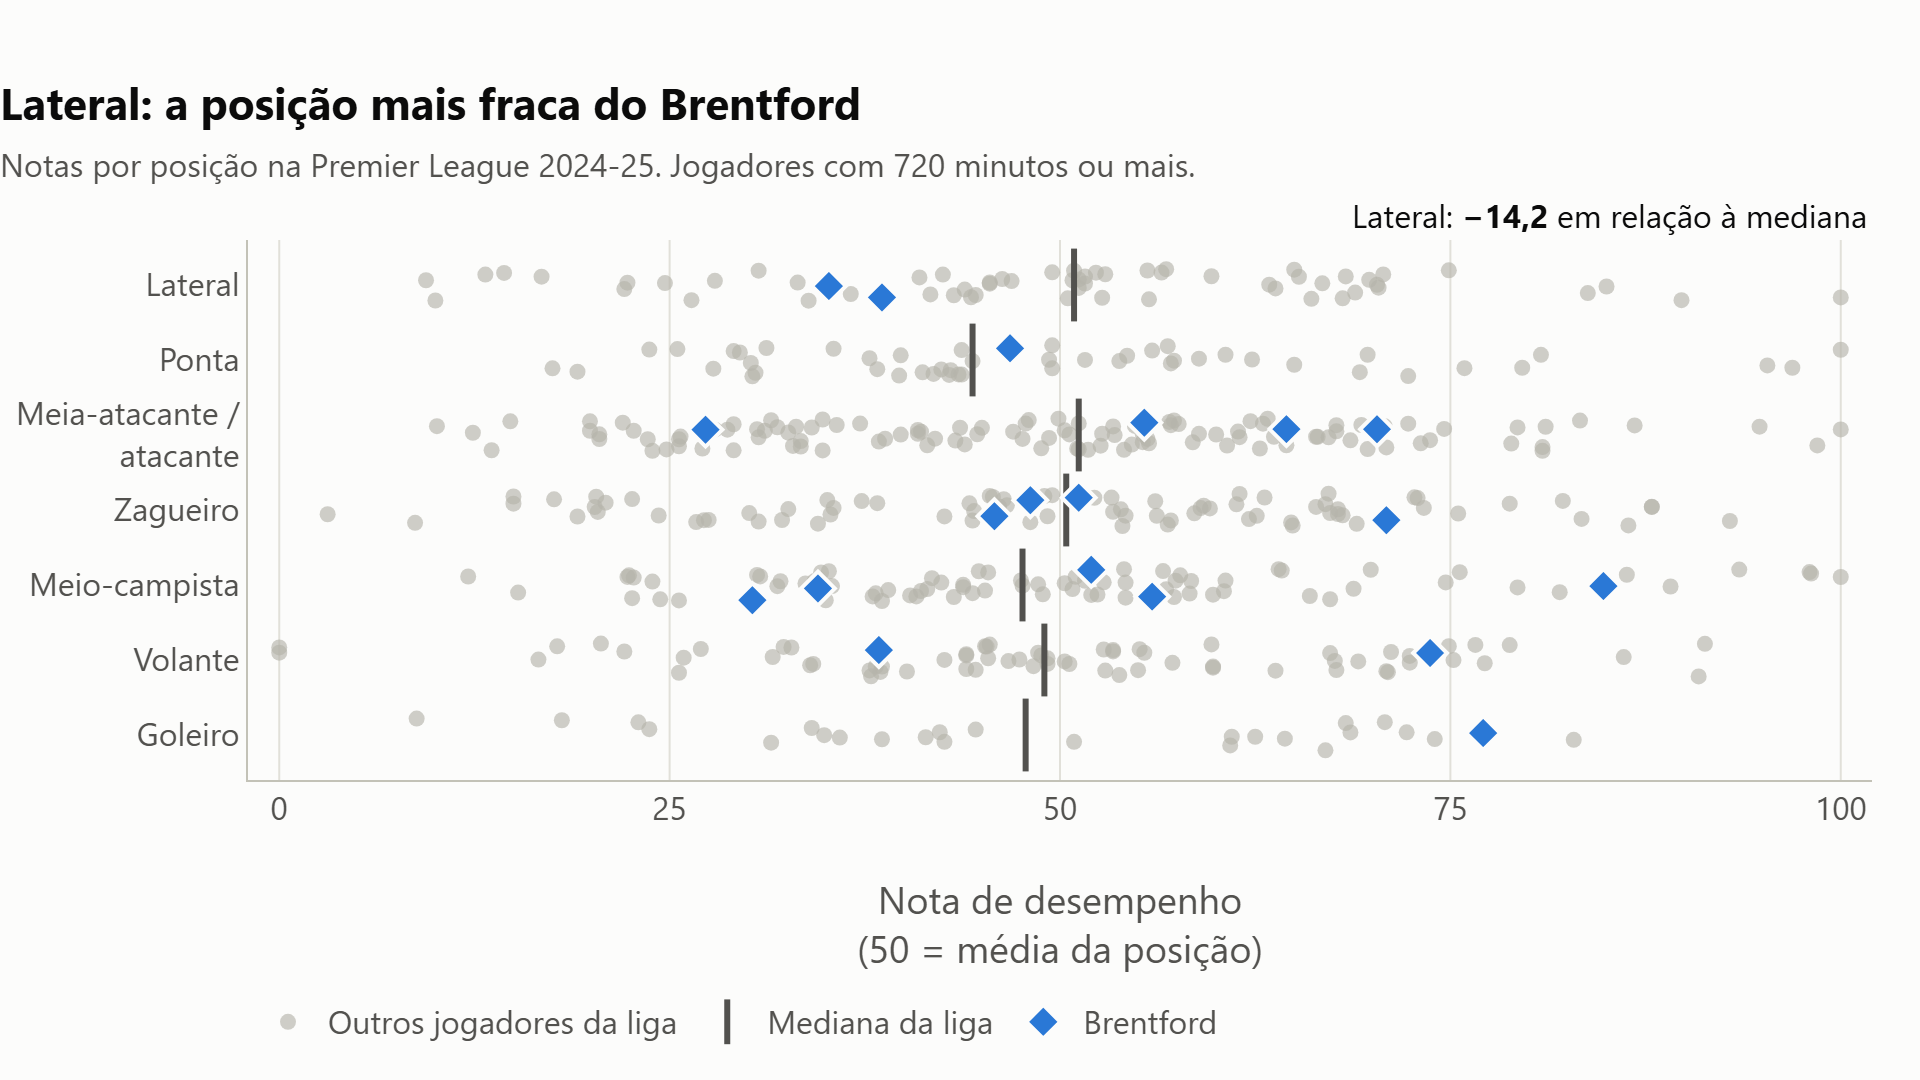
\includegraphics[width=0.86\linewidth]{fig1_diagnostico.png}
	\caption{Diagnóstico. Cada ponto cinza é um jogador da liga; cada losango azul é um jogador do Brentford; o traço escuro é a mediana da posição.}
	\label{fig:diagnostico}
\end{figure*}

\section{Mapeamento}

A Tabela~\ref{tab:mapeamento} liga cada dado à marca e ao canal visual que o representa. Em todos os gráficos, os valores principais ficam em \emph{posição sobre escala comum}, o canal em que o olho estima com mais precisão \citep{cleveland1984,munzner2014}; cor e forma só identificam o papel do jogador.

\begin{table}[t]
	\caption{Mapeamento dos dados para marcas e canais.}
	\label{tab:mapeamento}
	\footnotesize
	\centering
	\begin{tabular}{p{2.1cm}p{1.5cm}p{3.2cm}}
		\toprule
		Dado & Marca & Canal visual \\
		\midrule
		Nota do jogador & ponto & posição $x$ \\
		Posição em campo & faixa & posição $y$, ordenada pela diferença \\
		Papel do jogador & ponto & cor e forma (azul $\blacklozenge$, laranja $\bullet$, cinza) \\
		Valor de mercado & ponto & posição $x$, escala log \\
		Preço esperado & círculo vazio e traço & posição $x$; comprimento = desconto \\
		Orçamento, média do elenco & linha & posição fixa $x$ ou $y$ \\
		Percentil por métrica & ponto & posição $x$; peso define a ordem da linha \\
		\bottomrule
	\end{tabular}
\end{table}

\section{Representação visual}

\subsection{Diagnóstico: onde reforçar}

Pergunta: em qual posição o clube está mais abaixo da liga? A Figura~\ref{fig:diagnostico} mostra, para cada uma das sete posições, \emph{todos} os jogadores da liga como pontos sobre um eixo comum de nota, o traço da mediana e os jogadores do Brentford em destaque.

Por que este gráfico? A tarefa é comparar posições com a distribuição da liga. Uma barra com a média da posição esconderia a dispersão: veríamos que o lateral está abaixo, mas não que há poucos jogadores e que a liga inteira é muito espalhada. Mostrar cada jogador preserva essa incerteza.

Como ler? A posição mais fraca fica no topo e em negrito, e as demais descem da pior para a melhor. O valor ao lado do nome é a diferença para a mediana: lateral $-14{,}2$, enquanto o goleiro está em $+29{,}3$. Ordenar pela diferença faz o problema do clube ser a primeira coisa que se vê. Só a posição horizontal (a nota) carrega informação: a altura de cada ponto dentro da faixa é um deslocamento aleatório pequeno (\emph{jitter}), usado para que jogadores com notas parecidas não se sobreponham e para que a densidade da liga apareça. O sorteio usa semente fixa, então figura e painel mostram a mesma disposição.

\subsection{Mercado: quem contratar}

Pergunta: quem tem desempenho bom e preço baixo, dentro do orçamento? A Figura~\ref{fig:mercado} cruza valor de mercado (eixo $x$) e nota (eixo $y$) para os jogadores da posição nos clubes com dados de valor.

Por que este gráfico? Duas variáveis quantitativas e a procura por quem se destaca da nuvem pedem um diagrama de dispersão. Mais importante, as regras de indicação viram geometria:
\begin{itemize}
	\item a linha vertical é o orçamento (\eur{25}): quem está à esquerda cabe nele;
	\item a linha horizontal azul é a nota média do elenco (36,7): quem está acima é melhor que o atual;
	\item o traço laranja de cada indicado vai do preço atual (círculo cheio) ao preço esperado pelo modelo (círculo vazio): quanto mais longo, maior o desconto.
\end{itemize}
Djed Spence e Neco Williams ficam acima da linha azul, à esquerda da vertical, com traços longos. Spence custa cerca de \eur{20} e o modelo esperaria cerca de \eur{42}; Williams, de forma parecida. O leitor confere as três regras sem abrir uma tabela.

Escala logarítmica. O eixo é logarítmico (ticks em 5, 10, 20 e 50) e isso está escrito no título do eixo, porque a escala logarítmica engana quem não percebe que as distâncias são razões. Ela também é a escala em que o modelo de preço foi ajustado, então o traço do desconto mede a mesma coisa que o modelo calcula.

\begin{figure*}[t]
	\centering
	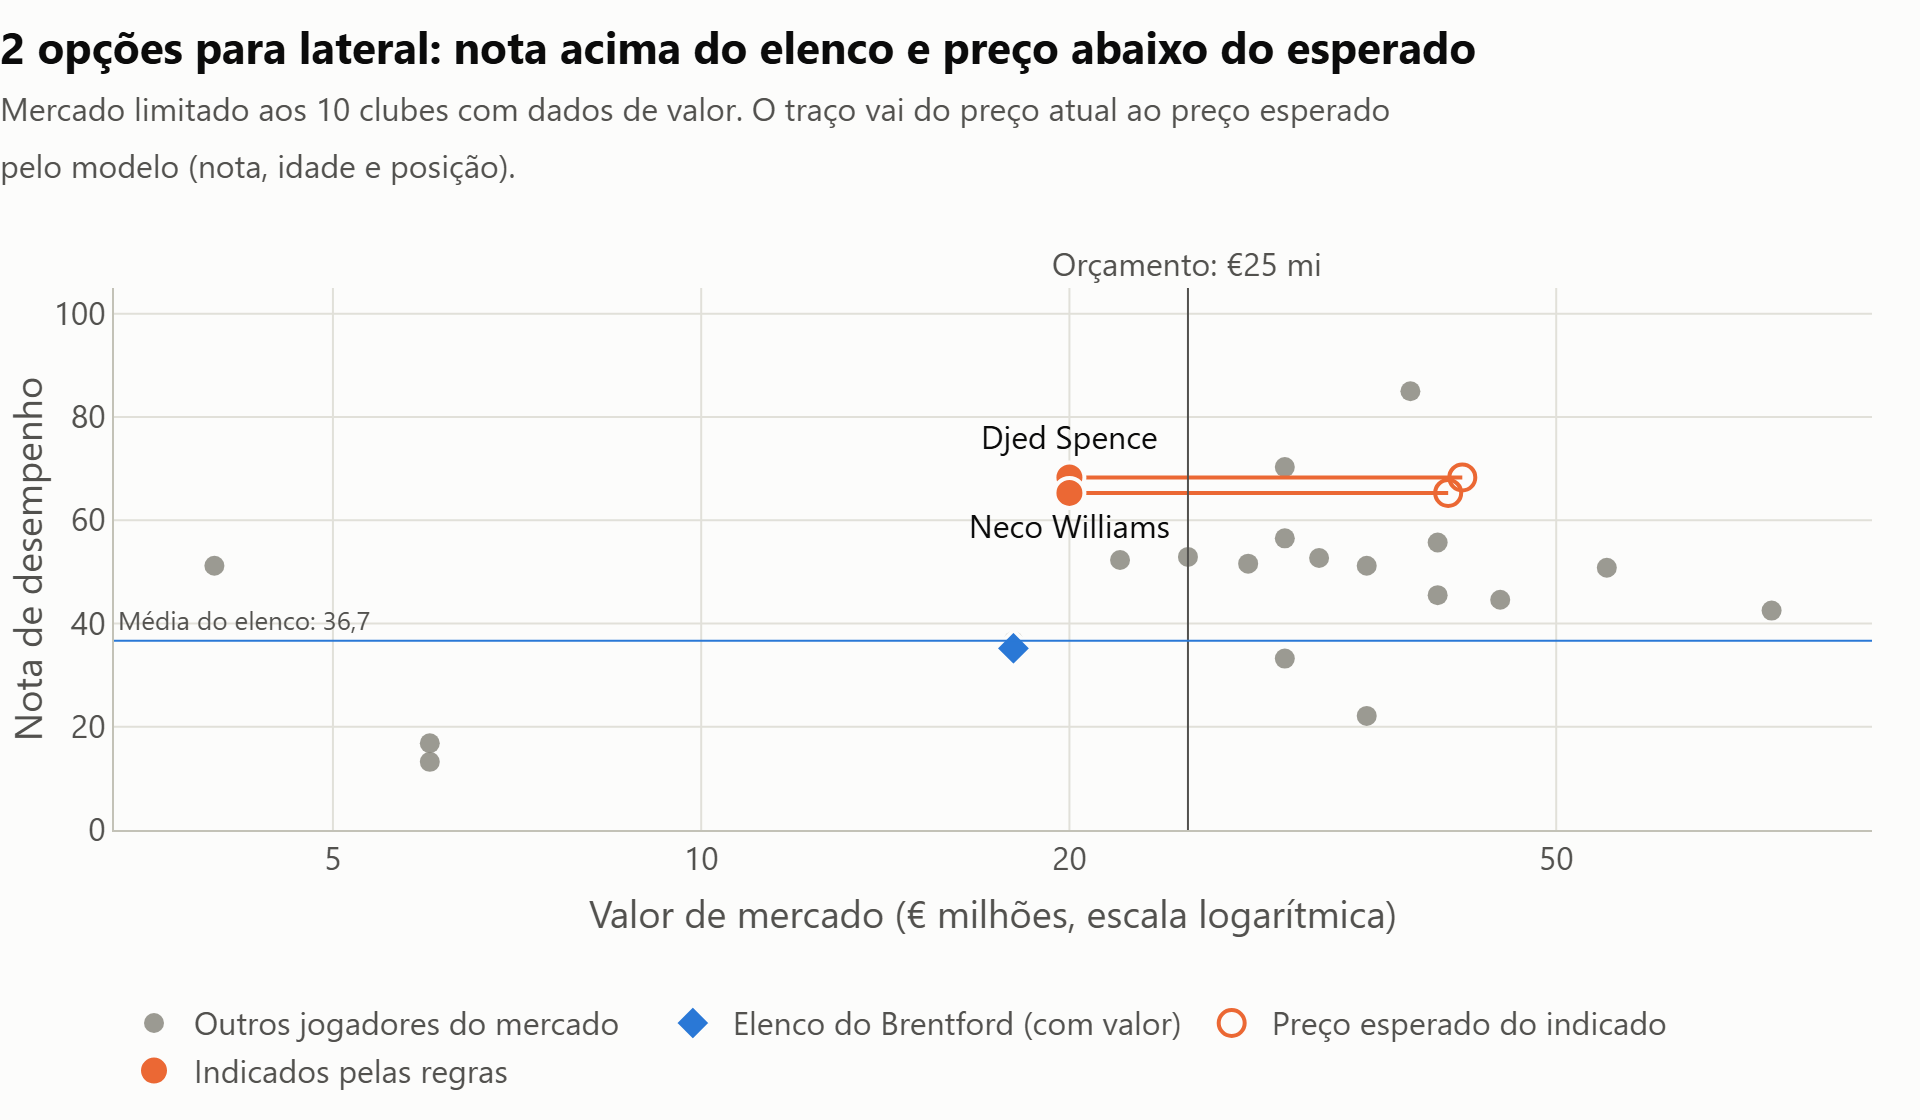
\includegraphics[width=0.86\linewidth]{fig2_mercado.png}
	\caption{Mercado. Orçamento (linha vertical), média do elenco (linha azul) e preço esperado de cada indicado (círculo vazio) tornam visíveis as três regras de indicação.}
	\label{fig:mercado}
\end{figure*}

\subsection{Decisão: o preço compensa?}

Pergunta: o candidato é melhor que o titular atual, e em quê? A Figura~\ref{fig:decisao} compara Djed Spence com Kristoffer Ajer, o jogador do Brentford com mais minutos na posição, em percentis da posição, uma linha por métrica.

Por que este gráfico? O objetivo é comparar dois valores por métrica. Um gráfico de pontos ligados (\emph{dumbbell}) coloca os dois jogadores na mesma linha e na mesma escala, e o traço entre eles mede a diferença diretamente \citep{cleveland1984}. As métricas vão da mais pesada à menos pesada, com o peso no rótulo, de modo que as diferenças que mais importam para a nota aparecem no topo. O laranja fica à direita do azul em todas as seis linhas, e o título diz: seis de seis.

Percentil como escala. O percentil na posição leva métricas de unidades diferentes para uma escala comum de 0 a 100, em que 100 é sempre o melhor, \emph{inclusive nas métricas negativas}, que são invertidas. A mediana (percentil 50) é uma linha de referência.

\subsection{Radar: perfil de um jogador (painel)}

Na aba de jogadores, o painel mostra um radar com os percentis de um único jogador sobre a mediana tracejada. O radar é controverso, e por isso foi limitado: aparece \emph{só um jogador} e \emph{sem preenchimento}, pois a área do polígono depende da ordem dos eixos. Para comparar dois jogadores, o painel usa o gráfico da Figura~\ref{fig:decisao}. O valor exato do percentil é impresso em negrito em cada eixo, porque ler um número num anel é mais difícil que ler o número impresso.

\begin{figure*}[t]
	\centering
	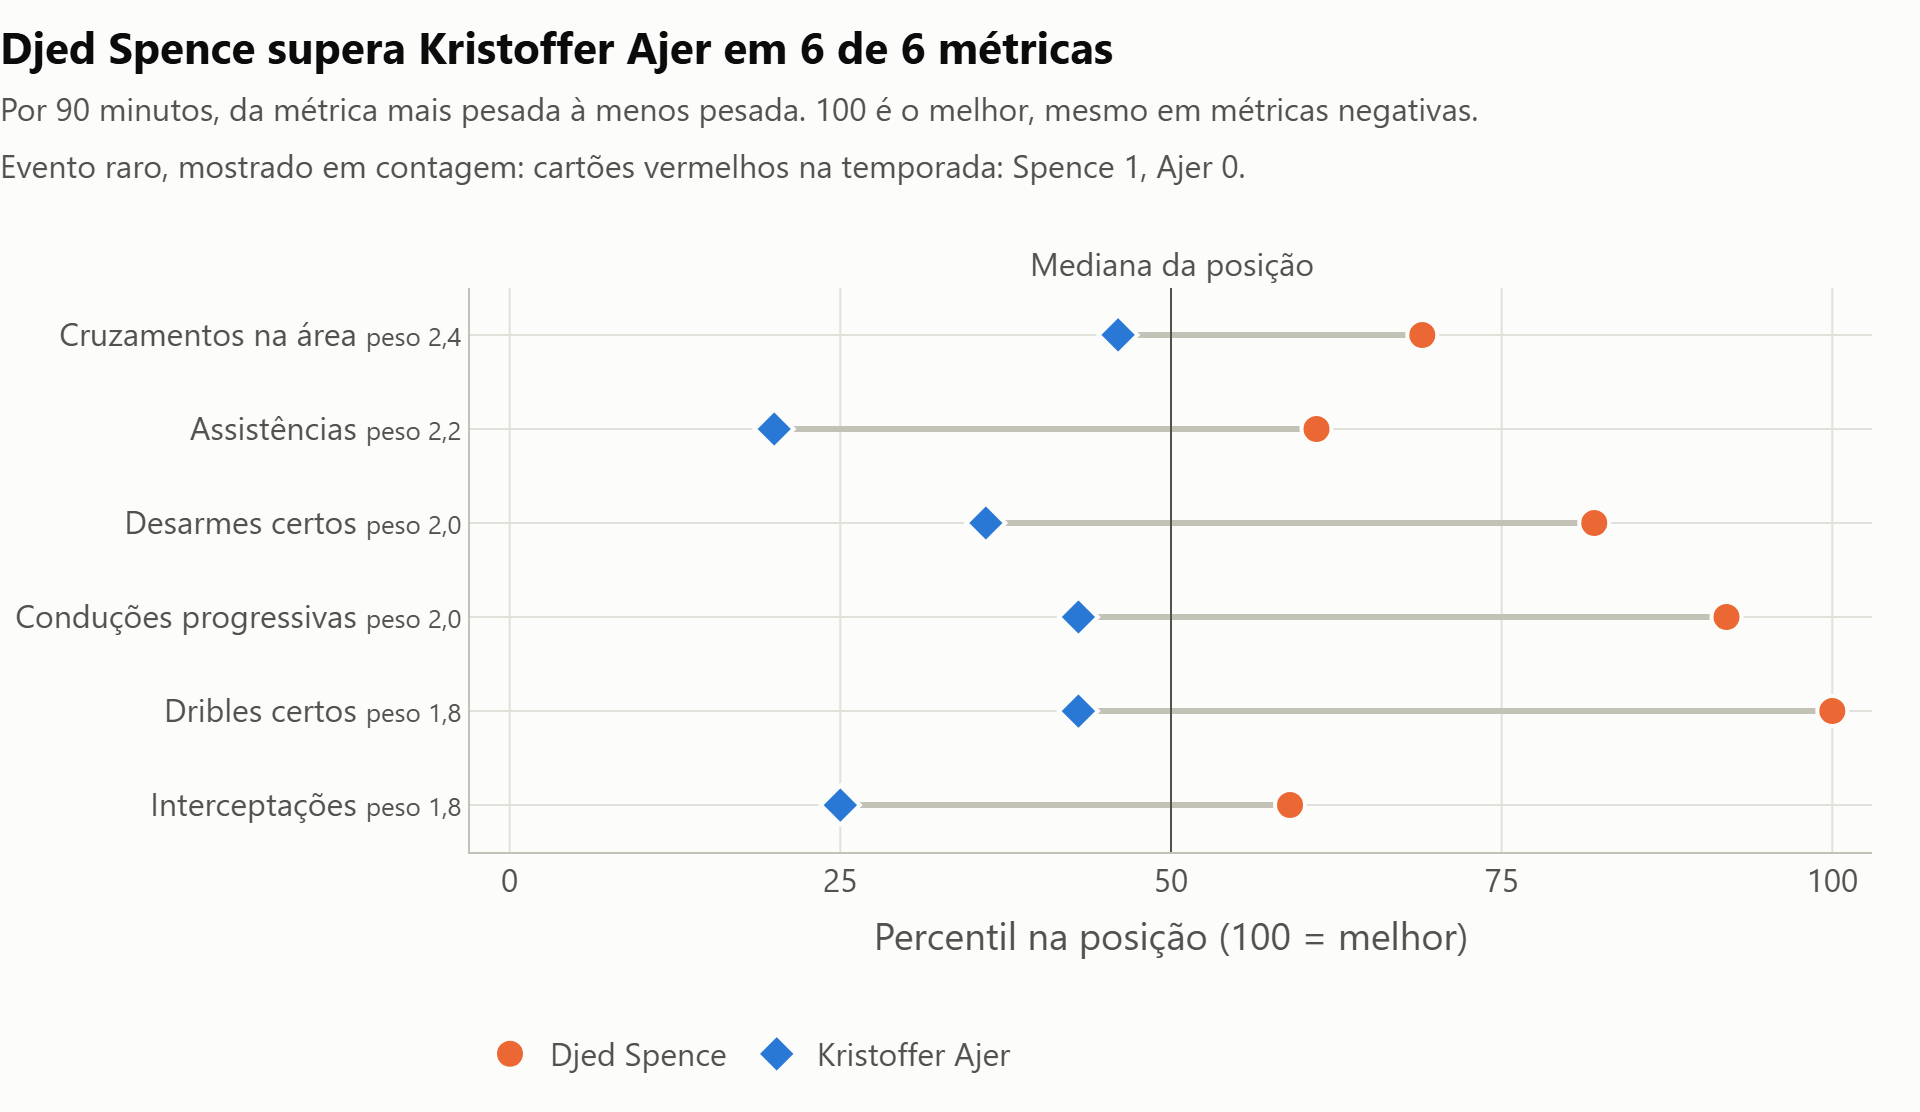
\includegraphics[width=0.86\linewidth]{fig3_decisao.png}
	\caption{Decisão. Percentil de cada jogador em cada métrica; o traço entre os pontos é a diferença. Cartões vermelhos aparecem como contagem no subtítulo.}
	\label{fig:decisao}
\end{figure*}

\subsection{Parâmetros padrão que foram trocados}

Os padrões do Plotly servem para exploração rápida, mas não para uma figura de decisão. A Tabela~\ref{tab:padroes} lista os principais ajustes.

\begin{table*}[t]
	\caption{Parâmetros padrão alterados e o motivo.}
	\label{tab:padroes}
	\footnotesize
	\centering
	\begin{tabular}{p{2.5cm}p{4.0cm}p{4.0cm}p{4.6cm}}
		\toprule
		Elemento & Padrão & Ajuste & Motivo \\
		\midrule
		Tema & modelo \texttt{plotly} com fundo azulado e grade forte & \texttt{template="none"}, grade clara, fundo uniforme & remover tinta sem informação \citep{tufte1983} \\
		Cinza de contexto & claro (\#b5b3ab) & escurecido (\#8a887f) & atingir contraste 3:1 com o fundo \citep{wcag2018} \\
		Marcadores & todos círculos de mesma cor & losango azul, círculo laranja, borda na cor do fundo & redundância cor+forma; borda separa pontos sobrepostos \\
		Eixo de valor & linear & logarítmico, ticks 5, 10, 20, 50 & distribuição assimétrica; mesma escala do modelo \\
		Limites dos eixos & ajuste automático & $[-2,102]$ e $[-3,103]$ & marcadores em 0 e 100 não são cortados \\
		Posição vertical (diagnóstico) & pontos empilhados na mesma linha & dispersão vertical (\emph{jitter}) de $\pm0{,}22$, semente fixa & evitar sobreposição sem mexer no valor $x$ \\
		Título & título simples, centralizado & título em negrito à esquerda, com subtítulo & título afirma a conclusão; subtítulo explica a leitura \\
		Legenda & à direita, fora do foco & horizontal, abaixo do eixo & não rouba largura do gráfico \\
		Separadores numéricos & ponto decimal & \texttt{separators=",."} e sinal ``$-$'' & padrão do leitor brasileiro \\
		Eixo radial do radar & números sobre os anéis & anéis a cada 25, valor em negrito em cada eixo & leitura direta, sem cálculo sobre o anel \\
		Fonte e tamanhos & 12 px & 16 px (base) e 13 px (notas) & legibilidade ao reduzir a figura para a coluna \\
		\bottomrule
	\end{tabular}
\end{table*}

Cinza do contexto. A primeira versão usava um cinza claro que ficava abaixo de 3:1 de contraste e quase sumia no papel. Escurecê-lo tornou o contexto legível sem competir com o azul e o laranja, as únicas cores saturadas. Dispersão vertical. Sem ela, os jogadores de uma posição ficam sobrepostos na mesma linha; ela é aplicada só ao eixo vertical (a posição já é categórica) e com semente fixa, para a figura ser a mesma a cada geração. Margens. Títulos de duas linhas colidiam com o gráfico, então a margem superior passou a crescer com o número de linhas do subtítulo.

\subsection{O que mudou depois da auditoria}

Uma revisão às boas práticas de visualização mudou cinco coisas:
\begin{itemize}
	\item Barras $\to$ pontos ligados. A comparação entre dois jogadores era um gráfico de barras agrupadas. Como o que interessa é a diferença, e não a magnitude de cada valor, os pontos ligados são mais diretos.
	\item Radar de um só jogador, sem área. A versão anterior sobrepunha dois polígonos preenchidos.
	\item Eventos raros fora dos percentis. Em cartões vermelhos, gols contra e erros, quase todos têm zero, e um único cartão derrubaria o jogador para perto do percentil 3. Esses eventos aparecem como \emph{contagem} no subtítulo (Spence 1, Ajer 0), e o título conta ``6 de 6'' métricas, as plotadas.
	\item Regras desenhadas no mercado. A média do elenco e o preço esperado, citados no título, foram adicionados ao gráfico.
	\item Diferença ao lado do rótulo. No diagnóstico, o número passou a acompanhar o nome de cada posição.
\end{itemize}

\section{Análise dos dados}

Lidas em sequência, as figuras contam uma história. O diagnóstico mostra que o lateral é a posição mais fraca do Brentford, $-14{,}2$ pontos abaixo da mediana, enquanto o goleiro está $+29{,}3$ acima. O mercado mostra que, com \eur{25}, só dois laterais cumprem as três regras: Djed Spence e Neco Williams, ambos com nota acima da média do elenco (36,7) e preço bem abaixo do esperado. A decisão mostra que Spence supera o titular Kristoffer Ajer em todas as seis métricas plotadas, com a maior diferença em dribles certos e conduções progressivas.

Os gráficos também expõem os limites da análise:
\begin{itemize}
	\item Cobertura. Só 10 dos 20 clubes têm valores conhecidos em número suficiente, e o gráfico de mercado diz isso no subtítulo.
	\item Modelo de preço. Ele explica 55\% da variação do valor, e a idade sozinha explica 47\%. O erro típico é de 1,68 vez, por isso só há indicação quando o desconto supera esse erro.
	\item Nota e preço. Em goleiros, zagueiros e volantes a nota tem relação nula ou negativa com o preço, então o gráfico de mercado deve ser lido com mais cautela nessas posições.
	\item Lateral. A diferença de $-14{,}2$ vem de apenas dois jogadores e varia de $-2{,}3$ a $-14{,}2$ conforme quem conta como lateral.
	\item Valor não é custo. O valor de mercado é uma estimativa, e não o preço real da transferência.
\end{itemize}

\section{Takeaways}

\begin{itemize}
	\item Sobre os dados: o lateral é o ponto fraco do Brentford, e Spence e Williams são os dois nomes que as regras indicam com \eur{25}. É um ponto de partida para o \emph{scouting}, e não uma recomendação final.
	\item Sobre o projeto: cada gráfico responde a uma tarefa: comparar com a distribuição (pontos sobre escala comum), procurar quem se destaca (dispersão logarítmica) e medir a diferença entre dois candidatos (pontos ligados).
	\item Sobre a eficácia: o que torna os gráficos úteis é menos a técnica do que a disciplina: codificação fixa e redundante, regras desenhadas, títulos que afirmam a conclusão e parâmetros padrão trocados quando atrapalhavam a leitura.
	\item Sobre a honestidade visual: eventos raros, incerteza e limites dos dados ficam visíveis, em vez de escondidos.
\end{itemize}

\section{Análise de viabilidade}

É possível extrair um produto: o painel em Streamlit já faz isso, pois permite escolher clube, posição e orçamento e refaz os três gráficos e os cartões dos jogadores. Seria útil como primeiro filtro de \emph{scouting}, antes da análise de vídeo e da conversa com os clubes. Três pontos limitam o uso real:
\begin{itemize}
	\item Dados. Os termos de uso do FBref e do Transfermarkt ainda não foram verificados, então a base não é redistribuída no repositório.
	\item Cobertura. Hoje o painel só funciona em 10 clubes. Ampliar exige mais valores de mercado.
	\item Contexto tático. A nota mede produção estatística, e não função tática. Defensores de times dominantes podem ficar subavaliados.
\end{itemize}
O código é genérico em relação ao clube e à posição, então estender a outras ligas depende mais de dados do que de novos gráficos.

%	REFERÊNCIAS
\printbibliography[title={Referências}] % Print the bibliography, section title in curly brackets


\end{document} % FIM DO DOCUMENTO
